\documentclass[10pt]{article}
\usepackage[a4paper, total={6.9in, 9.4in}]{geometry}
\usepackage{graphicx}
\usepackage{wrapfig}
\usepackage{hyperref}
\usepackage{fancyhdr}
\usepackage[font=it]{caption}
\graphicspath{ {./img/} }
\usepackage{titlesec}
\titleformat{\section}[block]
{\normalfont\Large\bfseries}{\thesection.}{1em}{}

\begin{document}

\begin{titlepage}

    \begin{center}
        \vspace*{1cm}
        \Huge
        \textbf{Clothing FaQTory}\\
        \LARGE
        \textbf{Object Oriented Programming Project}\\
        \vspace{1cm}
        \Large
        Elena Ferro\\
        \large
        \#2042328

        \vspace{10cm}

        \includegraphics[width=0.25\textwidth]{unipd.png}

        \Large
        \vspace{1cm}
        University of Padua\\
        \vspace{0.3cm}
        {\large Computer Science\\}
        \vspace{0.3cm}
        Academic year 2023/23

    \end{center}
\end{titlepage}
\tableofcontents
\newpage
\pagestyle{fancy}
\fancyhead[R]{Elena Ferro - 2042328}
\fancyhead[L]{Clothing FaQTory}
\section{Introduction}
ClothingFaQTory is a management software designed for a company that produces
clothing items and accessories. The core functionalities it provides are
managing an inventory of the different types of products and calculating their
production cost. Its aim is to help managers and business analysts to establish
the final selling price of the aforementioned items.

The calculation is based on the cost of the prime materials per unit (such as
the price of denim per meter) which is then multiplied by the approximate
surface of the final product, in order to estimate the quantity of material
needed.

The price is not stored with all the other information: the cost of the
materials is rather dynamic over time, being influenced by economy and other
factors. Therefore, the software allows to easily change the cost of the prime
materials and obtain an immediate recalculation of the product prices, without
having to update all the records in the database. In a real world scenario,
with possibly thousands of products, this operation would be really onerous.

I chose this topic because the calculation of the price for each concrete
product is the perfect circumstance to adopt polymorphism.

\section{Logic model}
The logic model is subdivided in two parts: the products hierarchy itself,
whose diagram is shown in \hyperref[fig:accessoriesUML]{Figure 1} and Figure
\hyperref[fig:clothingItemsUML]{Figure 2} (splitted for reasons of space), and
all the classes to interact with the database and handle errors, described in
the \hyperref[sec:dataPersistance]{data persistance section}.

The products hierarchy represents all the items that the company sells. Each of
them has generic information, such as \texttt{color}, \texttt{description},
\texttt{size}, etc. An alphanumeric code is also associated to each product.
The code is not unique, since the software offers the possibility to store
different variations of the same product (for instance, two items with the same
code could be manufactured in different colors).

A product can be either an \texttt{Accessory} or a \texttt{ClothingItem}. Both
of them are implemented by three concrete classes, each of which has additional
data to compute the final price (this data can either be a static constant,
such as the \texttt{DIAMETER} of the \texttt{Hat} class, or a dynamic and
instance-dependant value, such as the \texttt{capacity} in liters of a
\texttt{BackPack}). A very basic case of this calculation is the price of
\texttt{Jeans}, obtained with the sum of the lateral area of two cilinders. On
the other hand, a more elaborated example would be the \texttt{Bracelet} (which
is composed of a number of X pearls, each with a diameter of Y). Its cost is
computed through the volume of each pearl (approximately a sphere) multiplied
by the specific weight of the pearl's material.

A diamond inheritance case has been inserted in the hierarchy:
\texttt{Overalls} are considered to be a composition of the top part (a
\texttt{Vest}) and the bottom part (a pair of \texttt{Jeans}). Hence, the final
price is the sum of both its parents cost.

The \texttt{Size} of the product affects the final price too: a clothing item
of larger size obviously requires more material than a smaller one, therefore
the manufacturing cost is higher. A percentage, named
\texttt{extraPercentageOfMaterial}, is assigned to each size. This represents
how much extra material is needed to fabricate an element of that size compared
to the smallest size. For instance, if the field
\texttt{extraPercentageOfMaterial} for the size \texttt{M} is set to 20, it
means that a clothing item of size \texttt{M} requires $20\%$ more material to
be produced than one of size \texttt{XS} (which is the smallest). This
percentage is supposed to be constant over time.

\texttt{Product},
\texttt{Size} and \texttt{Material} all extend the \texttt{Model} class, which
represents a generic database entity and only exposes the \texttt{id} field.
The \texttt{id} is set to -1 by default, which is to mean that the record has
not been created yet.
\\\linebreak
Two custom containers have been created for the hierarchy entities;
the first one is \texttt{Map<K, V>}, which stores ordered key-value
pairs. Likewise \texttt{std::map}, it is based on a self-balancing red-black
tree and thus provides efficient search, insert and delete operations in $O(\log n)$ time.
Its main usages are holding the products subdivided by their concrete
type and supporting a rudimentary caching system in \hyperref[sec:repositoryPattern]{\texttt{SizeRepository}
    and \texttt{MaterialRepository}}, which simply stores in a map the
entities that have already been retrieved by id, to avoid repeatedly quering
the database for the same data.

Since some functions of \texttt{Map}, such as \texttt{keys()} and
\texttt{values()}, needed a list-like container, I also implemented a plain
\texttt{LinkedList<T>} container, to make \texttt{Map} independent from
\texttt{std::list}.

\begin{figure}
    \centering
    \includegraphics[scale=0.155]{accessories_uml.png}
    \caption{Logic model class UML (Accessories part)}
    \label{fig:accessoriesUML}
\end{figure}
\begin{figure}
    \centering
    \includegraphics[scale=0.165]{clothing_items_uml.png}
    \caption{Logic model class UML (ClothingItems part)}
    \label{fig:clothingItemsUML}
\end{figure}
\pagebreak

\section{Polymorphism}
One of the uses of polymorphism is the implementation of the Visitor design
pattern, through the \texttt{VisitorInterface} class. It allows performing
different operations on the hierarchy, depending on their dynamic type. This
interface is extended by three different concrete classes. Two of them are used
to build different UI layouts: \texttt{InfoDialogVisitor}, to display a dialog
with the complete product information, and \texttt{SpecificProductInfoVisitor}
to populate the form for items creation and editing. The third usage is the
\texttt{FieldGetterVisitor}, which takes a \texttt{Product} subclass as a
parameter and creates a key-value map between its field names and their current
value. This comes in handy in different circumstances: in the aforementioned
dialog to show the product information, but also to export the entities as JSON
and to dynamically build the database \texttt{INSERT} queries.

With the purpose of dumping data to files, the Decorator design pattern has
been utilized, coupled with the aforementioned \texttt{FieldGetterVisitor}. The
\texttt{JSONExportableDecorator} class (extending \texttt{DecoratorInterface})
enriches the \texttt{Model} class adding the functionality to export an entity
as a \texttt{QJsonObject}, while keeping the hierarchy itself totally
independent from any QT class (and thus potentially reusable with another
framework).

Other examples of polymorphism are the computation of the product price,
different for each concrete \texttt{Product} class, and the implementation of
the Repository pattern (illustrated in the \hyperref[sec:dataPersistance]{data
    persistance section}), whose purpose is providing an abstraction layer between
the data storage and the business logic.

Another significant example of polymorphism is the Strategy pattern. An
abstract \texttt{Mapper}\label{txt:Mapper} defines the blueprint for an
algorithm used to map query results, from \texttt{QSqlQuery} to a generic
\texttt{Model*}. For each entity, a concrete class extending \texttt{Mapper}
and overriding \texttt{operator()} has been defined.

The project is based on a Model-View-Controller architecture. Views and
Controllers are totally independent from the data source, hence the possibility
to effortlessly substitute the data source (for instance, with an API
integration) leaving the frontend code entirely untouched.

\section{Data persistance}
\label{sec:dataPersistance}
The chosen method for data persistance is a PostgreSQL database. The primary
motivation for this choice is that Postgres natively supports both single and
multiple hierarchy between tables and is generally more efficient than
other DBMS, such as MySQL.

The database structure is therefore symmetrical to the C++ hierarchy, having
the table \texttt{product} as a parent to all the others, with foreign keys
referencing the \texttt{size} and \texttt{material} tables.

The Entity-Relationship diagram and the schema of the database can both be
found in the project files, inside the \texttt{docs} directory.

Postgres connections become idle after a certain timeout of inactivity, which
obviously results in the inability to use the software. To overcome this
problem without having to set an unnecessarily large timeout, the
\texttt{ConnectivityManager} class regularly pings the database every minute.
To avoid slowing down the other operations, this is done in a separate thread.

\subsection{Repository pattern}
\label{sec:repositoryPattern}
In order to interact with the database, the Repository pattern has been
implemented. A UML class diagram for this pattern can be found inside the
\texttt{docs} directory.

The \texttt{Repository} class is abstract, and only exposes static utility
functions to execute queries and check for errors. It is then extended by
\texttt{ReadOnlyRepository<T>} and \texttt{DeleteOnlyRepository}, whose common
child is \texttt{CRUDRepository<T>}.

Each concrete repository implements the Singleton pattern, which means that
just a single instance will be created, and then referenced everywhere.

This structure provides different types of concrete repositories. For instance,
\texttt{SizeRepository} is read-only since its records will not be modified. Oh
the other hand, the only operations carried out directly on the
\texttt{product} table \texttt{DELETE} queries and given that the record can be
deleted equally from the parent or child table, \texttt{DeleteOnlyRepository}
is used.

Repositories for each \texttt{Product} subclass must support CRUD operations.
Consequently, a concrete repository extending and specializing at the same time
\texttt{CRUDRepository<T>} has been implemented for each one of them.

The concrete repository instantiations take care of passing the correct table
name and \hyperref[txt:Mapper]{\texttt{Mapper}} to its parents. Furthermore, in
an hypothetical extension of this project, it might become necessary to have a
specific query for a given entity. With separated concrete repositories, this
method can conventiently be implemented in the corresponding concrete class,
preserving the separation of concerns. This last described mechanism is
inspired by Java's \href{https://hibernate.org/}{Hibernate}
library.\\\linebreak Another layer of abstract is added through the
\texttt{QueryBuilder} utility. No repository class uses directly SQL statements
as strings, since this is error-prone, but rather composes them chaining calls
to the \texttt{QueryBuilder} methods and executing \texttt{.build()} in the end
(which returns the composed string).

\subsubsection{Error handling}
Repositories also checks the query for errors. Being the use of exceptions
highly debated in C++, I preferred to implement a functional-languages-inspired
error handling strategy: each function returns an object of type
\texttt{Either<Error, Entity>}, which contains an \texttt{Error} if it has
occurred, otherwise the requested entity. The \texttt{Either} class offers
methods to check if the contained value, stored in a \texttt{std::variant}, is
right (thus the query was successfull) or left (the query resulted in an error)
and the method \texttt{fold}, which accepts two lambda functions,
\texttt{ifLeft} and \texttt{ifRight}.

If an error was detected, the controller which called the repository method
will take care of handling it, emitting a \texttt{databaseError} signal,
received by the respective \texttt{View}.

\section{Implemented features}
The following list includes additional features, compared to those strictly
required.
\subsection{Functional}
\begin{itemize}
    \item Export entities as JSON, divided by type
    \item Filter the products by type, code or price range (and eventually combine these
          filters)
    \item Sort the products by available quantity, sold quantity or code
    \item Obtain an esteem of the products price
    \item Validation of all the forms (in the filter panel, in the wizard to create and
          edit the products and in the dialog to set the material price)
\end{itemize}

\subsection{Graphical}
\begin{itemize}
    \item Usage of a tab bar to distinguish between operations on the \texttt{product}
          hierarchy and on the \texttt{material} table.
    \item Usage of a toolbar in the Products tab to provide \texttt{Create new},
          \texttt{Filter} and \texttt{Export to JSON} functionalities, with the
          respective keyboard shortcuts.
    \item Usage of a custom font.
    \item Usage of stylesheet to personalize the tab bar and the buttons in the materials
          cost tab.
    \item Usage of icons in the tab bar, toolbar, products tree view and materials cost
          tab.
    \item Usage of a tree view widget to display the products divided by product type.
          When expanded, the general information for the items is shown, together with
          icon buttons to edit, delete and view also the specific product information
          (not shown in the main view). A square icon with the preview of the product
          color is also created for each row.
    \item Asking confirmation through a dialog before deleting a product
    \item Button to clear all the filters (appears only when filters are applied).
          \pagebreak
    \item Wizard to create and edit the products:
          \begin{itemize}
              \item Possibility to generate a random code during the creation process (clicking
                    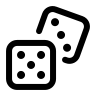
\includegraphics[width=12pt,height=12pt]{dices.png} beside the code
                    field).
              \item Select the color of the product with the color picker widget. Once the color is
                    picked a preview of the color and its hex code will be available, with the
                    button text adapting to the background, in order to be readable with both dark
                    and light colors.
              \item Keyboard shortcuts to navigate the wizard pages.
              \item Validation of the mandatory form fields, which turn red if the user tries to
                    click next but they are not filled.
              \item Based on the chosen product type, the user will be prompted to insert the
                    specific fields for that product (in addition to the generic information common
                    to all the items).
          \end{itemize}

\end{itemize}
\newpage
\section{Hours report}
\begin{table}[h]
    \centering
    \begin{tabular}{|l|c|c|}
        \hline
        \textbf{Activity}                          & \textbf{Planned hours} & \textbf{Actual Hours} \\\hline
        Planning project structure                 & 5                      & 5                     \\
        Develop code for models and DB interaction & 12                     & 14                    \\
        Study QT framework                         & 8                      & 11                    \\
        UI code development                        & 15                     & 16                    \\
        Testing and debugging                      & 6                      & 8                     \\
        Report                                     & 4                      & 4                     \\\hline
        \textbf{Total}                             & 50                     & \textbf{58}           \\\hline
    \end{tabular}
\end{table}
As shown in the table, the project required 8 extra hours to be completed as
compared to the initial evaluation. This is attributable to the necessity to
deepen my knowledge of QT regarding both classes to interact with the database
and UI widgets, but also to introduce graphical improvements such as custom
icons and font and optimize the mapping of entities from queries.
\end{document}